\section{Performance evaluation and testing}

\subsection{Testing}
A proper testing is needed for ensure the implementation work, before applying optimisation's and performance evaluation. I tested the runtime with the programs given, \texttt{tparallel.c}, \texttt{ttask.c} and \texttt{tsynchtasks.c}. Which where used during the development and when the final build is done, checking, it leads, to correct result.

\par ~\\
Also some algorithms where used for the testing. The first one was the mandelbrot set. I used the code given to check the output match. I modified the source code so it worked with the miniomp implementation (no single after parallel pragma needed) the version is called \texttt{tmandel-mini.c} and another version that works with the openmp implementation with name \texttt{tmandel-omp.c}. The following process was done to check the output matches:

\begin{figure}[h!]
    \centering
    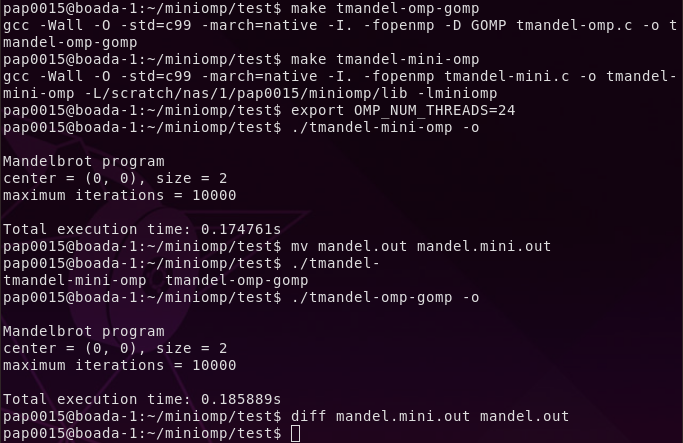
\includegraphics[width=0.9\textwidth]{mandelcheck.png}
    \caption{Check process for mandelbroot code}
\end{figure}
\par ~\\
At this point we can tell that our implementation works well, but as a more strict testing is needed, I wrote a sample code to test all capabilities of the implementation.

\subsection{Tool for scalability analysis}
For performance evaluation purposes, I developed a tool that given to executables, one linked to miniomp and the other linked to openmp. The script can be found at \texttt{test} folder in the root of the miniomp project. I will not be explaining the script as it is out of the scope of this document. 


